\section{Quantum Error Correcting Code}
\lecture{20 May}

\subsection{Mathematical Fundamentals to Quantum Information / Computation}
First off, some basics to the mathematics of quantum theory. The following description to the quantum theory is an overly simplified one, with plenty of its historical backgrounds missing, leaving only the essential mathematical results. And as always, don't forget that ``all models are wrong, but some are useful." The mathematical formulation to quantum mechanics has evolved for a hundred years, and it is, to this date, the most successful mathematical description we have of our observed world. It doesn't mean that is how the world actually works, but just that the mathematics checks out with the experiment that we cared about and can actually conduct.

In quantum information science, the most basic information-carrying unit is a qubit, which is described by a trace-1 positive semi-definite operator $\rho$ termed the density operator acting on the vector space $\mathbb{C}^2$. With multiple qubits combined, we obtain a quantum system. When we have multiple qubits, say $\rho_1$ and $\rho_2$, the combined systems is described by a larger density operator $\rho_1\otimes\rho_2$, acting on the combined vector space.

An experiment / measurement conducted on a quantum system is a partition of unity: each event $i$ is described by a positive semi-definite operator $E_i$ satisfying
\begin{equation}
    \sum_i E_i = \mathbbm{1}.
\end{equation}

When conducting the experiment $E=\{E_i\}$ on a system $\rho$, the probability of seeing the outcome $i$ is defined by the Born rule:
\begin{equation}
    \mathrm{Pr}\{i\} = \trace{E_i\rho} \in [0,1].
\end{equation}
Some often used measurements are $\{\ket{0}\bra{0},\ket{1}\bra{1}\}$ and $\{\ket{+}\bra{+},\ket{-}\bra{-}\}$, where a \textit{bra} vector is $\bra{x} \defeq \ket{x}^\dagger$, and the \textit{ket} vectors of the computational basis are defined as $\ket{0} \defeq [1,0]^\transpose$, $\ket{1} \defeq [0,1]^\transpose$, and $\ket{\pm} \defeq \frac{1}{\sqrt{2}}(\ket{0} \pm \ket{1})$. If two vectors are tensored together, we simply denote it by concatenation, i.e., $\ket{00}=\ket{0}\otimes\ket{0}$.

The evolution of a quantum system is unitary, viz., for a state $\rho$ evolving through a quantum system, there exists a unitary $U$ such that
\begin{equation}
    \rho \mapsto U \rho U^\dagger
\end{equation}
represents the evolution.

For further understanding of the mathematics behind quantum information science, one should refer to any other book but this note.

\subsection{Quantum Error Correcting Code}
Our task is to protect our density operator $\rho$ from close-to-identity unitary evolutions / noises. When applying the $\{\ket{+}\bra{+},\ket{-}\bra{-}\}$-measurement, the probability of obtaining the outcome $+$ should be
\begin{equation*}
    \mathrm{Pr}\{+\} = \trace{\ket{+}\bra{+}\rho} = \bra{+}\rho\ket{+}.
\end{equation*}
However, under a unitary noise $U$, the result will in turn be
\begin{equation*}
    \bra{+}U \rho U^\dagger\ket{+}.
\end{equation*}

Our first attempt to correct this is to duplicate $\rho$, say into three copies. If $U$ happens with a probability of $3\%$, then with the three copies, we can use majority voting and reduce the error probability to $1\%$.

But we can do much better by utilizing the \textit{entanglement} nature of the quantum theory. Again given three qubits, we can thus construct density operators of size $8\times 8$. For example, the state
\begin{equation}
    \rho = \frac{1}{2}\left[\begin{matrix}
        1 \\ & 0 \\ & & 0 \\ & & & 0 \\ & & & & 0 \\
        & & & & & 0 \\ & & & & & & 0 \\ & & & & & & & 1
    \end{matrix}\right] = \frac{1}{2} \left(\ket{000}\bra{000} + \ket{111}\bra{111}\right) \label{eq:w14_repetition_code_density_operator}
\end{equation}
is a repetition code, whereas
\begin{equation}
    \rho = \frac{1}{4}\left[\begin{matrix}
        1 \\ & 0 \\ & & 0 \\ & & & 1 \\ & & & & 0 \\
        & & & & & 1 \\ & & & & & & 1 \\ & & & & & & & 0
    \end{matrix}\right] = \frac{1}{4} \left(\ket{000}\bra{000} + \ket{011}\bra{011} + \ket{101}\bra{101} + \ket{110}\bra{110}\right)
\end{equation}
is a parity check code.

This is essentially what quantum error correcting code (QECC) is! We encode our usual codes within quantum states.

Of course, our encoding need not be in the $\{\ket{0},\ket{1}\}$ basis, we can have
\begin{equation}
    \rho = \frac{1}{4}\left[\begin{matrix}
        1 & 0 & 0 & 1 & 0 & 1 & 1 & 0 \\
        0 & 1 & 1 & 0 & 1 & 0 & 0 & 1 \\
        0 & 1 & 1 & 0 & 1 & 0 & 0 & 1 \\
        1 & 0 & 0 & 1 & 0 & 1 & 1 & 0 \\
        0 & 1 & 1 & 0 & 1 & 0 & 0 & 1 \\
        1 & 0 & 0 & 1 & 0 & 1 & 1 & 0 \\
        1 & 0 & 0 & 1 & 0 & 1 & 1 & 0 \\
        0 & 1 & 1 & 0 & 1 & 0 & 0 & 1
    \end{matrix}\right] = \frac{1}{2} \left(\ket{+++}\bra{+++} + \ket{---}\bra{---}\right).
\end{equation}

\begin{figure}[t]
    \centering
    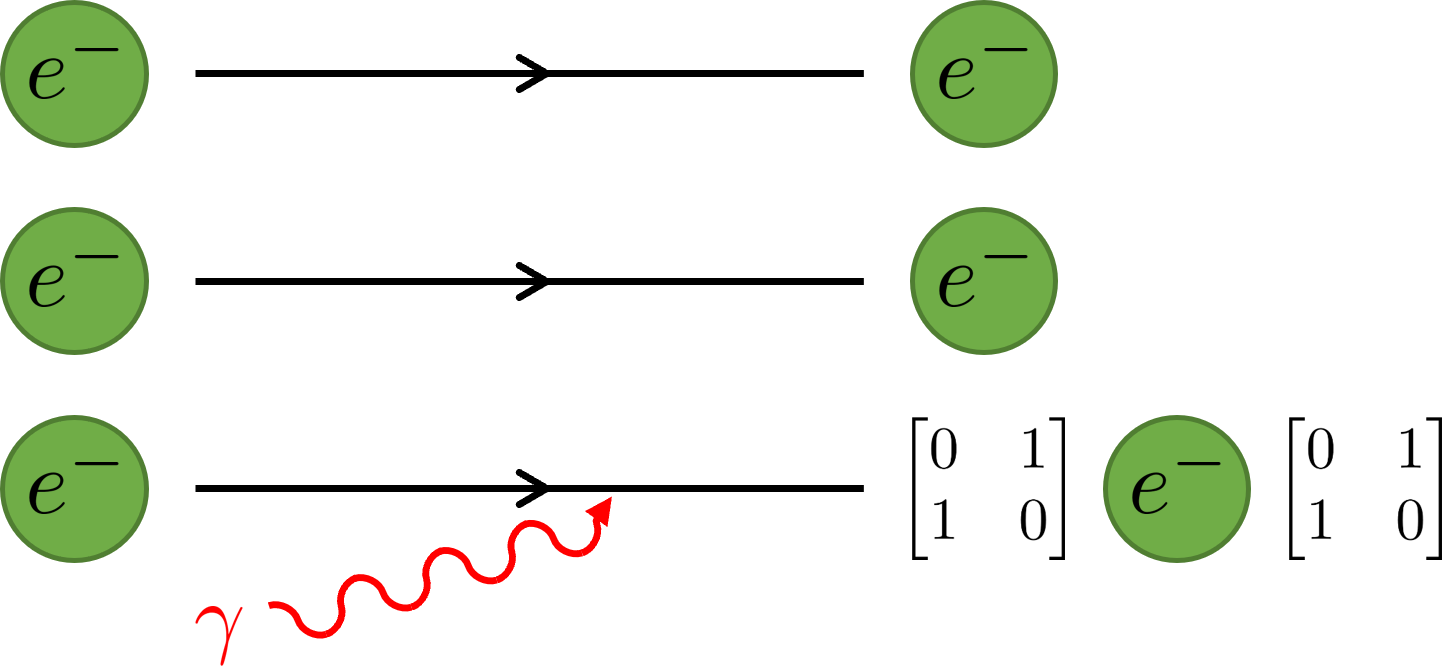
\includegraphics[width=0.5\linewidth]{figures/w14_quantum_bit_flip.png}
    \caption{Bit flip of a quantum system. Each qubit is represented by an electron $e^-$. The third qubit is hit by an incident photon $\gamma$ that changes the state by the unitary matrix $X$.}
    \label{fig:w14_quantum_bit_flip}
\end{figure}

A kind of noise that often occurs is a bit flip by a photon, see \autoref{fig:w14_quantum_bit_flip}. The unitary gate caused by an incident photon acting on the third qubit is the Pauli-X gate:
\begin{equation}
    X \defeq \left[\begin{matrix}
        0 & 1 \\ 1 & 0
    \end{matrix}\right],
\end{equation}
which is also known as the NOT gate as it satisfies
\begin{equation}
    X\ket{0} = \ket{1},\; X\ket{1} = \ket{0}.
\end{equation}
The total unitary that acts on the 3-qubit system is
\begin{equation}
    U = \mathbbm{1}\otimes\mathbbm{1}\otimes X = \left[\begin{matrix}
        0 & 1 \\
        1 & 0 \\
        && 0 & 1 \\
        && 1 & 0 \\
        &&&& 0 & 1 \\
        &&&& 1 & 0
    \end{matrix}\right].
\end{equation}

Assume the input state is the repetition code density operator as described in \autoref{eq:w14_repetition_code_density_operator}, how, then, do we detect and fix the error induced? Consider the following quantum circuit in \autoref{fig:w14_fix_bit_flip}.

\begin{figure}[H]
    \centering
    % \includegraphics[width=0.5\linewidth]{}
    \caption{Fixing a bit flip error.}
    \label{fig:w14_fix_bit_flip}
\end{figure}

If the first measurement turns out to be



%%%%%%%%%%%%%%%%%%%%%%%%%%%%%%%%%%%%%%%%%%%%%%%%%%%%%%%%%%%%%%

\section{Database}
Here we discuss the \textit{relational databases} $R(X,Y)$. Given